\documentclass[letterpaper,12pt]{article}
\usepackage{array}
\usepackage{threeparttable}
\usepackage{geometry}
\geometry{letterpaper,tmargin=1in,bmargin=1in,lmargin=1.25in,rmargin=1.25in}
\usepackage{fancyhdr,lastpage}
\pagestyle{fancy}
\lhead{}
\chead{}
\rhead{}
\lfoot{}
\cfoot{}
\rfoot{\footnotesize\textsl{Page \thepage\ of \pageref{LastPage}}}
\renewcommand\headrulewidth{0pt}
\renewcommand\footrulewidth{0pt}
\usepackage[format=hang,font=normalsize,labelfont=bf]{caption}
\usepackage{listings}
\lstset{frame=single,
  language=Python,
  showstringspaces=false,
  columns=flexible,
  basicstyle={\small\ttfamily},
  numbers=none,
  breaklines=true,
  breakatwhitespace=true
  tabsize=3
}
\usepackage{amsmath}
\usepackage{amssymb}
\usepackage{amsthm}
\usepackage{harvard}
\usepackage{setspace}
\usepackage{float,color}
\usepackage[pdftex]{graphicx}
\usepackage{hyperref}
\hypersetup{colorlinks,linkcolor=red,urlcolor=blue}
\theoremstyle{definition}
\newtheorem{theorem}{Theorem}
\newtheorem{acknowledgement}[theorem]{Acknowledgement}
\newtheorem{algorithm}[theorem]{Algorithm}
\newtheorem{axiom}[theorem]{Axiom}
\newtheorem{case}[theorem]{Case}
\newtheorem{claim}[theorem]{Claim}
\newtheorem{conclusion}[theorem]{Conclusion}
\newtheorem{condition}[theorem]{Condition}
\newtheorem{conjecture}[theorem]{Conjecture}
\newtheorem{corollary}[theorem]{Corollary}
\newtheorem{criterion}[theorem]{Criterion}
\newtheorem{definition}[theorem]{Definition}
\newtheorem{derivation}{Derivation} % Number derivations on their own
\newtheorem{example}[theorem]{Example}
\newtheorem{exercise}[theorem]{Exercise}
\newtheorem{lemma}[theorem]{Lemma}
\newtheorem{notation}[theorem]{Notation}
\newtheorem{problem}[theorem]{Problem}
\newtheorem{proposition}{Proposition} % Number propositions on their own
\newtheorem{remark}[theorem]{Remark}
\newtheorem{solution}[theorem]{Solution}
\newtheorem{summary}[theorem]{Summary}
%\numberwithin{equation}{section}
\bibliographystyle{aer}
\newcommand\ve{\varepsilon}
\newcommand\boldline{\arrayrulewidth{1pt}\hline}
\begin{document}

% ----------------------------------------------------------------------
\begin{flushleft}
  \textbf{\large{Problem Set \#4}} \\
  MACS 30100, Dr. Evans \\
  Chih-Yu Chiang \\
  Python Version: 3.5.2
\end{flushleft}
\vspace{5mm}
\noindent\textbf{Problem 1} \\
\\
The minimization processes in the 2 estimations of (c) and (d) both succeeded.
For acquiring converged results from the algorithms, the estimation settings are as follow: \\
(c). error simple mode = False; minimization method = L-BFGS-B. \\
(d). error simple mode = False; minimization method = TNC. \\

\noindent\textbf{Part (a). histogram} \\
\\
A histogram of annual incomes of students who graduated in 2018, 2019, and 2020 from the University of Chicago M.A. Program in Computational Social Science. \\
\begin{figure}[htb]\centering\captionsetup{width=6.0in}
  \caption{\textbf{}}
  \fbox{\resizebox{4.0in}{3.0in}{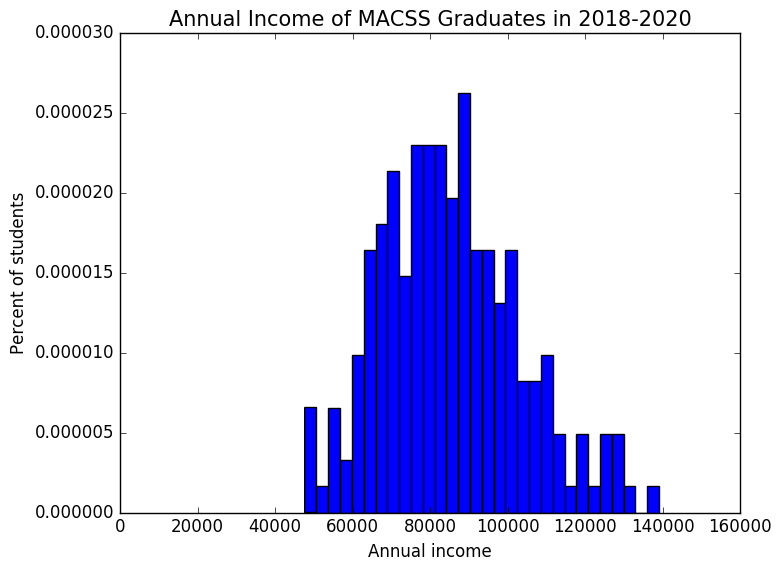
\includegraphics{1a.png}}}
\end{figure} \\

\noindent\textbf{Part (b). lognormal pdf function} \\
\\
With $\mu$ = 5.0 and $\sigma$ = 1.0, and xvals = np.array([[200.0, 270.0], [180.0, 195.5]], \\
The lognormal PDF values are [[0.0019079, 0.00123533], [ 0.00217547, 0.0019646]].
\\


\clearpage

% ----------------------------------------------------------------------
\noindent\textbf{Part (c). One step SMM with mean and std} \\
\\
One step SMM is estimated with mean and standard deviation as moments and identity weighting matrix. The initial guess of $\mu$ is 11 and $\sigma$ is 0.2, with 300 simulations and 200 observations each.\\
The criterion value is 7.20176828929e-14. The estimated parameters are as follows:
\[\mu_{SMM1}= 11.3307149892\]
\[\sigma_{SMM1}= 0.208868329657\]

\begin{center}
\begin{tabular}{ c|c|c }
 moments & mean & std \\
 \hline
 data & 85276.8236063 & 17992.542128 \\
 model & 85276.8464227 & 17992.5419414 \\
 (data-model)/data & -2.67557875682e-07 & 1.03738379265e-08
\end{tabular}
\end{center}
\\

A lognormal pdf with estimated parameters is plotted. \\

\begin{figure}[htb]\centering\captionsetup{width=6.0in}
  \caption{\textbf{}}
  \fbox{\resizebox{4.in}{3.0in}{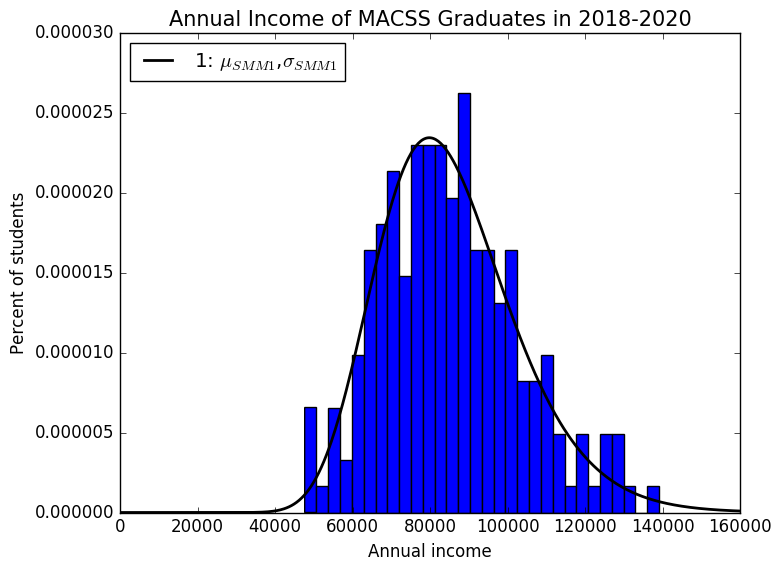
\includegraphics{1c.png}}}
\end{figure} \\

\clearpage

% ----------------------------------------------------------------------
\noindent\textbf{Part (d). Two step SMM with mean and std} \\
\\
Two step SMM is estimated with mean and standard deviation as moments and weighting matrix derived from (c). The initial guess of $\mu$ and $\sigma$ is the estimated results from (c). \\
The criterion value is 0.0120239766133. The estimated parameters are as follows:
\[\mu_{SMM2}= 11.3307146745\]
\[\sigma_{SMM2}= 0.208868331657\]

\begin{center}
\begin{tabular}{ c|c|c }
 moments & mean & std \\
 \hline
 data & 85276.8236063 & 17992.542128 \\
 model & 85276.8196196 & 17992.5364623 \\
 (data-model)/data & 4.67498781548e-08 & 3.14895601719e-07
\end{tabular}
\end{center}
This is really close to the result from (c). While the data and model moment differences are both trivial and the criterion values can't be compared with different weighting matrices, it's hard to say, the result from (c) and (d), which one is better.
\\

Lognormal pdfs with estimated parameters in previous and this questions are plotted. \\

\begin{figure}[htb]\centering\captionsetup{width=6.0in}
  \caption{\textbf{}}
  \fbox{\resizebox{4.0in}{3.0in}{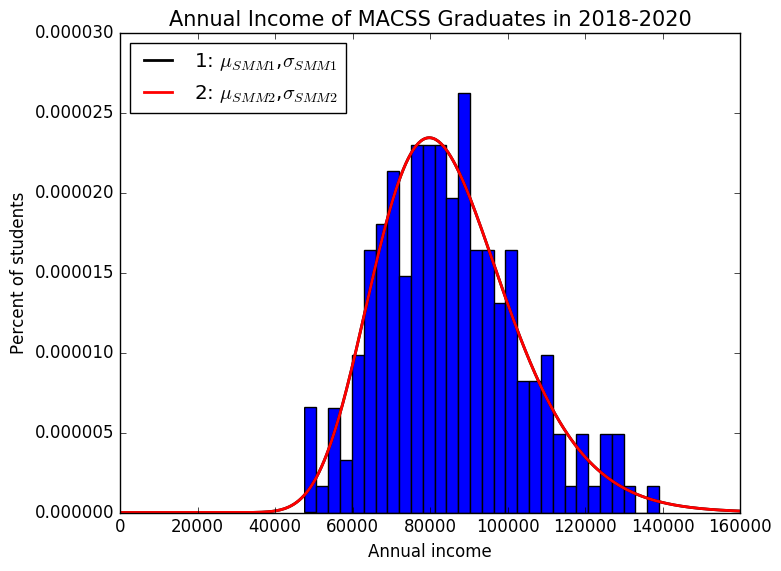
\includegraphics{1d.png}}}
\end{figure} \\


\end{document}
